
% CHAPTER:  1
% (Note: cannot have a footnote on a word within the \chapter{} construct, it does not work)
\newcommand{\s}{$_{\rm s}$}
\newcommand{\kms}{km~s$^{-1}$}
\newcommand{\msun}{{\it M}$_{\odot}$}
\newcommand{\lsun}{{\it L}$_{\odot}$}
\newcommand{\mear}{{\it M}$_{\oplus}$}
\newcommand{\etal}{{\it et al.}}
\newcommand{\ie}{{\it i.e.}}
\newcommand{\eg}{{\it e.g.}}
\newcommand{\be}{\begin{equation}}
\newcommand{\ee}{\end{equation}}
\newcommand{\magarc}{{\rm mag\,arcsec$^{-2}$}}
\newcommand{\MK}{{{\rm M}_{\rm ext,K}-5\log h}}
\newcommand{\ri}{{$r_{21}$}}
\newcommand{\ra}{$R_A$}
\newcommand{\vobs}{{v_{\rm obs}}}
\newcommand{\kmsMpc}{km~s$^{-1}$ Mpc$^{-1}$}
\newcommand{\h}{$h_{70}$}
\newcommand{\vpec}{v_{\rm pec}}
\newcommand{\like}{{\mathcal L}}
\newcommand{\vs}{\vspace*{5pt}}
\newcommand{\continued}{ (Continued)}

\newcommand{\ferengi}{\textsc{ferengi}}
\newcommand{\hst}{\textit{HST}}
\newcommand{\hubble}{\textit{Hubble Space Telescope}}
\newcommand{\subaru}{\textit{Subaru}}
\newcommand{\sextractor}{\textsc{SExtractor}}
\newcommand{\galapagos}{\textsc{Galapagos}}
\newcommand{\galfit}{\textsc{GALFIT}}
\newcommand{\gimtwod}{\textsc{GIM2D}}
\newcommand{\sersic}{S\'{e}rsic}






% Galaxy Zoo
\newcommand{\ffeatures}{$f_{\rm features}$}
\newcommand{\ffeaturesz}{$f_{\mathrm{features,}z}$}
\newcommand{\ffeaturesrest}{$f_{\mathrm{features,}z=0.3}$}
\newcommand{\ffeaturesdebiased}{$f_{\mathrm{features,debiased}}$}
\newcommand{\fbest}{$f_{\mathrm{features,best}}$}
\newcommand{\fodd}{$f_{\mathrm{odd}}$}
\newcommand{\fbar}{$f_{\mathrm{bar}}$}
\newcommand{\fclumpy}{$f_{\mathrm{clumpy}}$}
\newcommand{\fsmooth}{$f_{\rm smooth}$}
\newcommand{\fartifact}{$f_{\rm artifact}$}

\newcommand{\fHI}{f_{\rm HI}}
\newcommand{\zsim}{$z_{\mathrm{sim}}$}

% Bands

\newcommand{\Bband}{$B_{435W}$}
\newcommand{\Vband}{$V_{606W}$}
\newcommand{\iband}{$i_{775W}$}
\newcommand{\Iband}{$I_{814W}$}
\newcommand{\zband}{$z_{850LP}$}

% GZH subsamples

\newcommand{\main}{\texttt{main}}
\newcommand{\faded}{\texttt{faded}}
\newcommand{\recolored}{\texttt{recoloured}}
\newcommand{\goods}{\texttt{goods-shallow}}
\newcommand{\stripe}{\texttt{stripe-82-single}}
\newcommand{\coadd}{\texttt{stripe-82-coadd}}
\newcommand{\redshifted}{\texttt{redshifted}}
\newcommand{\simagn}{\texttt{simulated-agn}}




\chapter{UKIDSS}
\label{chap:ukidss}

\section{Intro: wavelength dependence on morphology: optical and IR}

Historically, visual morphological classification of galaxies has been conducted on optical images. Blue B-band images were the primary source dating back to Hubble's classic tuning-fork classification scheme \citep{Hubble1926} and in the subsequent modifications by \citet{Sandage1961} and \citet{DeVaucouleurs1963}. The more recent and larger morphological catalogs also derive their classifications from rest-frame optical images, either single-band (\citet{RC31991} (B-band), \citet{Scarlata2007} (ACS I-F814W), \citet{Fukugita2007} and \citet{Nair2010} (SDSS g-band)) or color-composite (\citet{Lintott2008}, \citet{Willett2013} (SDSS-gri)). 

In the optical regime, the flux is dominated by young, hot stars; this results in an emphasis of spiral structure in the images, but they tend to have patchy appearances due to the abundance of star-formation regions in the arms. Optical images also are impacted by extinction due to dust, which can obscure features that tend to be composed of older stellar components (such as bars and bulges). Longer wavelenths are free of these effects, making them ideal for revealing the underlying ``stellar backbone'' of galaxies.

It is possible, then, to consider two morphologically distinct components of a galaxy: a gas-dominated Population I disk, and a star-dominated Population II disk. The Population I disk is most easily seen in the optical, revealing HII regions, cold HI gas, and emission from young OB stars; these regions will tend to highlight flocculance in spiral structure. The Population II disk, on the other hand, traces the underlying mass distribution; consisting of the old, cooler stellar population, it is more easily seen at longer wavelengths. \citet{Block1999} even suggests that two separate classifications schemes should be required for all galaxies; one for the Population I disk, which can be probed in optical and ultraviolet images, and a Population II disk, for which longer wavelength images, free of dust extinction, would be required. 

The extent to which the morphologies of the younger and older stellar populations are decoupled, however, is not yet clear. Early studies which directly compared optical and near-IR images found very significant differences between the two morphologies \citep{Hackwell1983,Thronson1989,Block1991,Block1994}. \citet{Block1999} goes as far as to sugget that there is no correlation between the two, and that the optically-definied Hubble tuning fork ``does not constrain the morphology of the old steallar Population II disks.'' However, all of the aforementioned studies only compared morphologies of either a single galaxy, or at most a handful, so these conclusions cannot be applied generally.

The advent of larger surveys incorporating near and mid-IR detectors enabled morphological comparisons between the two wavelength regimes on a much grander scale than had previously been achieved. New results contradicted those of the previous case-studies: in general, IR morphology was found to be well-correlated with optical morphology in larger samples of galaxies. \citet{Eskridge2002} compared near-IR H-band (1.65$\mu$m) Hubble-type classifications to B-band in a sample of 205 nearby spiral galaxies from the Ohio State University Bright Spiral Galaxy Survey (OSUBSGS). Applying deVaucouler's classification system, they found an overall good correlation between the two morphologies, but on average galaxies from Sa through Scd appeared one T type earlier in the H band than in the B band. In the IR images the bulge tended to appear more prominent and the spiral arms less knotty, which resulted in the slightly earlier classifications. For the earliest (optically S0/a and Sa) and latest-type galaxies (optically Scd through Sm), no difference in morphologies was found. This is an expected result for the earlier-types, since these have little ongoing star formation and very little dust, so it is expected that both optical and IR morphologies are dominated by old stars. This result is less intuitive for the later-type galaxies, as these are dominated by ongoing star formation. However, these galaxies are defined as having very weak or nonexistant bulges and poorly defined spiral structure. Since the main driver in the differences in morphology across wavebands was found in the intermediate spirals to be the relative prevalance of a bulge and difference in contrast and appearance of spiral arms, galaxies lacking these features should not, in fact, be expected to look different in the IR than the optical. 
 
\citet{Buta2010} obtained similar results comparing optical and mid-IR (3.6 $\mu$m) images from the \textit{Spitzer} Survey of Stellar Structure in Galaxies ($\rm S^4G$, \citet{Sheth2010}) in a large sample of 2,331 spiral galaxies. Like \citet{Eskridge2002}, the optical and IR classifications were very well correlated, with the most significant differences occuring for S0/a to Sc galaxies, where the 3.6 $\mu$m were on average slightly earlier than the B-band classifications.

%Bars! 
%invisible in optical, visible in IR examples
Infrared imaging is also often used in place of (or in addition to) optical to indentify stellar bars (e.g. \citet{Mulchaey1997,Knapen2000,Block2004,Sheth2008}). Like bulges, bars are primarily composed of old, red stars, and therefore better traced by longer wavelengths. In fact, it is not uncommon for an infrared bar to be completely invisible in the optical. Notable examples include NGC 1566 \citep{Hackwell1983}, NGC 1068 \citep{Thronson1989,Scoville1988}, NGC 309 \citep{Block1991}, NGC 4736 \citep{Block1994}, and NGC 4303 (Figure 1, \citet{Sheth2003}). This trend is not only limited to case-studies; for example, in a larger sample of 29 galaxies classified as unbarred in the optical, \emph{50\%} of these were found to be barred in the near-IR images \citep{Mulchaey1997}.

%bigger: bar fraction
The fraction of spiral galaxies which exhibit bars (defined as the bar fraction) has been measured extensively in optical images, and typically falls near 50\% when bars of all strengths are considered \citep{Masters2010}(should probably cite more). Since it is much more common to find an infrared bar in an optically unbarred galaxy than the reverse, it is expected that the bar fraction in the infrared will, in general, be higher than what has been measured in the optical. Some studies find a substantial increase: \citet{Seigar1998} for example spectulate that ``bars may always be present in disks at some level'', based on finding a bar fraction of 90\% when using infrared images (as compared to their optical measurement of 68\%). Although their sample consisted of only 45 galaxies total, they claim this measurement should represent the general population of spirals, because their selection was not biased towards barred galaxies. Other studies report similar increases in bar fraction in the infrared, albeit not quite as large. \citet{Knapen2000} in a similar sample size of ~50 galaxies find a bar fraction in the infrared of ~70\%, a strong increase from the optical 50\%. \citet{Eskridge2000} in sample of 186 galaxies measure a bar fraction of 72\% in the infrared which is \emph{double} that of their optical measurement. While these studies report significant increases in bar fraction as a function of wavelength, they do dispute the claim by \citet{Seigar1998}, emphasizing that at least 30\% of galaxies in their sample are truly unbarred across all wavelengths.

%same bar fraction
Other more recent studies find larger bar fractions in the infrared, not significantly so. \citet{Whyte2002} measure an increase from 72\% to 79\% in a sample of 72 galaxies, while \citet{Sheth2008} reports 60\% for both wavelengths. \citet{MenendezDelmestre2007} also found a slight increase from 63\% to 67\% in a sample of 151 galaxies, noting that although bars tended to appear stronger in the near-IR, on average they were not so weak in the optical as to become undetectable. Finally, \citet{Buta2010} also reported a similar result of 60\% barred spirals, which was consistent with the fraction computed in optical RC3 classifications.

Now: segue into describing how we'll investigate these using a *much* larger sample than previously done, using GZ classifications. 2 goals: 1) investigate change in hubble-ish type in UKIDSS vs GZ2 (by looking at bulge question and arms-windyness), and 2) bar fraction, plus probably some case studies of galaxies whose morphologies change drastically.   

\section{UKIDSS sample}

The UKIDSS sample is comprised of 71,052 infrared images of galaxies which had been previously optically classified in GZ2. The images were taken with the United Kingdom Infrared Telescope (UKIRT) as part of the UKIRT Infrared Deep Sky Survey (UKIDSS; \citet{Lawrence2007,Warren2007}. The Large Area Survey (LAS) portion of UKIDSS covered the SDSS observations at high Galactic altitudes, allowing for full YZJHK coverage.  

Morphological classifications for the UKIDSS sample were obtained via Galaxy Zoo, where users were shown YJK color-composite images. The classification tree used was identical to that in GZ2, allowing a direct comparison of morphologies using the same vote fractions. Raw votes were counted and weighted by user consistency in the same manner as the GZ2 sample (details of this process are given in Chapter~\ref{chap:methodology}).

One major challenge in comparing the UKIDSS and GZ2 morphologies is to ensure that any differences measured are mostly driven by actual morphological differences between wavebands, and not due to varying instrumental parameters. Details of the instrumentation for both samples is shown in Table~\ref{tab:uk_gz2_instrumentation}. The resolution of both sets are comparible - with similar pixel size and PSF widths, the ability to resolve finer features in the images should be consistent for both. The difference in depth, however, is significant: the SDSS gri bands used to create the color-composite images in GZ2 are on average $\sim$1 magnitude deeper than what is achieved for the LAS YJK bands in UKIDSS. To minimize the impact the difference the difference in depth may have in comparing the two sets of images, the comparison sample is limited to the nearest and brightest galaxies. 
The sample is thus restricted to a volume-limit of $z<0.06$ and $M_{r,petro}<-20.0$, which consists of 10,395 galaxies of the 54,238 with spectroscopic redshifts.

\begin{center}
\begin{table}
\begin{tabular}{lcclc}
\hline \hline
\multicolumn{2}{c}{UKIDSS} & & \multicolumn{2}{c}{GZ2} \\
\cline{1-2}\cline{4-5}
Filter & Depth (AB mag) & & Filter & Depth (AB mag) \\

Y      & 21.13 & & g      & 22.2 \\
J      & 20.91 & & r      & 22.2 \\
K      & 20.25  & & i      & 21.3 \\
\cline{1-2}\cline{4-5}
seeing: & $<$1.2'' & & PSF width: & 1.4'' (median in r) \\
pixel scale: & 0.4'' & & pixel scale: & 0.396'' \\
\hline \hline
\end{tabular}
\caption{Comparison of depth and resolution of the UKDISS and GZ2 images. The resolution between the two surveys is comparable, but the UKIDSS images are an average of $\sim$1 magnitude shallower in all bands used to create the color-composite images that where classified. }
\label{tab:uk_gz2_instrumentation}
\end{table}
\end{center}

To further ensure that any observed difference in morphologies are due to physical (wavelength) dependencies, and not instrumentation, the sample is further restricted to only include galaxies for which the signal detected in the IR image extends to a significant fraction of the galaxy's total light profile. During preliminary visual inspection of side-by-side IR/optical images of the subjects, it was seen that for many of the optically-classified spirals, the arms in the IR images became so faint with respect to the bulge that there could be no fair comparison of morphologies using vote fractions. The two primary examples of this effect occured firstly in GZ2-classified spiral galaxies which the majority voted as ``smooth'' in UKIDSS, due to the bulge being the only visible feature in the IR images (see top row in Figure~\ref{fig:morph_change} for an example of this effect.). Second, for optically-barred galaxies whose spiral arms were undetectable in the IR, only the bar remained visible, giving it the appearance and classification of an edge-on galaxy (bottom row in Figure~\ref{fig:morph_change}). Not accounting for such cases could then give an underestimate of the total IR bar fraction.  

\begin{figure}
\centering
\includegraphics[width=\textwidth]{figures/morph_change.pdf}
\caption{Examples of two galaxies whose morphological changes between optical and IR wavelengths was driven by a lack of light detectable in the IR relative to optical. \textbf{Top}: A galaxy classified as featured and spiral in the optical using GZ2 vote factions, but smooth in the IR using UKIDSS vote fractions (dr7objid: 587726014553587781). \textbf{Bottom} A galaxy classified as featured and barred in the optical using GZ2 vote fractions, but due to the complete disappearance of arms in the IR, only the bar is visible, giving it the appearance and classification of an edge-on galaxy (dr7objid: 587734305416871963) }
\label{fig:morph_change}
\end{figure}


\subsection{S/N method for selecting equally-sized galaxies}

To identify which galaxies are sufficiently detected in both the IR and optical images, the S/N profile of the IR J-band images is compared to the r-band petrosian radius. For disk galaxies whose surface brightness distribution follows an exponential profile, 99\% of the galaxy's total flux is enclosed by the Petrosian magnitude \citep{Graham2005}, which is defined as the flux measured within two Petrosian radii. Therefore, we can let $2\times r_{petro}$ represent the radius that encloses the entire disk, which will be hereafter denoted as $r^{r}_{2petro}$. To properly compare morphologies of disk galaxies in IR and optical images, it must be ensured that a signal is detected in the J-band out to a significant fraction of that radius. This is done by computing the surface brightness profile in the J-band, and measuring the radius within which the S/N is greater than 3, which will be hereafter denoted as $r^{J}_{3}$. A cut is then placed on the volume-limited sample such that $r^{J}_{3} \ge 0.75  r^{r}_{2petro}$, which retains $\sim 60\%$, or 6,484 galaxies considered suitable for a robust morphological comparsion. The details of this process are described here. 


%J-band cutouts were downloaded directly using the WFCAM Science Archive\footnote{$\rm http://wsa.roe.ac.uk:8080/wsa/MultiGetImage\_form.jsp$}.% r-band cutouts were manually created for each galaxy using the DR7 bulk imaging fields obtained from the SDSS Data Archive Server\footnote{http://das.sdss.org/www/html/das2.html}. The default size of the cutouts (measured from the center to the edge) was set at 6 times the 90\% petrosian radius (\radr), to allow for sufficient measurement of the background. If the galaxy was within this distance from the edge of the bulk fits image, 2.0*\radr~was used. If the galaxy was still within this distance (and hence overlapped multiple SDSS frames), a proxy of $1.08\times\radr + 2.29''$ was used for the radius within which $S/N>5$. This proxy was derived from a linear fit to the radius within which $S/N>5$ vs \radr~for all galaxies where $r_{S/N>5}$ was derived directly from the $S/N$ profile, shown in Figure. This proxy was used for 10\% of the galaxies.
% 
%\begin{figure}
%\centering
%\includegraphics[width=.7\textwidth]{figures/rvr.pdf}
%\label{fig:rvr}
%\caption{Correlation between the 90\% petrosian radius in the r-band vs. the radius within which the signal-to-noise is greater than five ($r_{S/N>5}$). The linear fit was used to derive a proxy for $r_{S/N>5}$ for galaxies whose $S/N$ profiles could not be measured in the r-band.}
%\end{figure}
%

%The J-band fits images obtained were released in units of flux, while the r-band images were in counts. To convert the r-band images from counts to flux, 
%the following formula was used, as specified by the SDSS Photometric Calibration algorithm\footnote{$\rm http://classic.sdss.org/dr7/algorithms/fluxcal.html$}:

%\begin{equation}
%\rm f/f_{0}=(counts-1000)/exptime \times 10^{(aa+kk \times airmass)}
%\end{equation}

%where counts is the raw value from the fits image, exptime=53.907 is the exposure time for the images in seconds, aa and kk are the zeropoint and extinction coefficients located in the corresponding frame headers, in addition to the airmass. 1000 is subtracted from the counts to account for the ``softbias'' that is added to each pixel in DR7. 

The J-band cutouts were downloaded directly using the WFCAM Science Archive\footnote{$\rm http://wsa.roe.ac.uk:8080/wsa/MultiGetImage\_form.jsp$}. The signal to noise profiles are then computed on J-band sky-subtracted cutouts, where the sky subtraction is done using the \textsc{Python} package \textsc{photutils Background2D} function. %A \textsc{box\_size} of 3x3 was applied to all cutouts as this size would always be larger than the size of the source galaxy, as well as to ensure an integer number of boxes in both dimensions (which produces the best results according to the package documentation). 
The noise is defined as the dispersion in the background flux, shown in the top-left panel of Figure~\ref{fig:SN_calculation}. The background was fit to a Gaussian, and the noise was taken as the resulting standard deviation value given by the fit. The signal was computed by calculating the average flux per pixel within circular apertures of varying radii from the center of the galaxy to the edge of the cutout. From these a signal-to-noise profile was generated for each galaxy; an example is shown in the top-right panel of Figure~\ref{fig:SN_calculation}. The radius at which the $S/N$ profile falls below $S/N$=3 (or in other words, the radius within which the $S/N$ remains greater than 3, $r^{J}_{3}$), is recorded for each galaxy, represented as the green dashed line. The blue dashed line is drawn at $r^{r}_{2petro}$, representing the radius containing 99\% of the flux, as described above. The ratio of $r^{J}_{3}$ to $r^{r}_{2petro}$ is then used to evaluate whether the galaxy is sufficiently detectable in both wavelengths for a fair morphological comparison. The bottom row of Figure~\ref{fig:SN_calculation} shows the results of this method displayed on the color-composite images that are seen by GZ users. The circle on the optical image (left) shows $r^{r}_{2petro}$, and circle on the IR image (right) shows  the J-band radius within which $(S/N)_{J}>3,~r^{J}_3$. In this example, $r^{J}_{3}=0.62\times r^{r}_{2petro}$, indicating that the radius at which the galaxy is detectable in the J band is only 62\% that of what is visible in the r band. Given that the threshold for inclusion in the sample is $r^{J}_{3}/r^{r}_{2petro} \ge 0.75$, this galaxy is considered too faint in the IR with respect to the optical to fairly compare vote fractions.  




\begin{figure}
\centering
\includegraphics[width=.8\textwidth]{figures/SN_calculation_example.pdf}
\caption{Example of the $r^{J}_{3}$/$r^{r}_{2petro}$ calculation of one galaxy (dr7objid=587722981747392587). \textbf{Top Left}: The sky-subtracted background of the J-band images are fit to a Gaussian to derive the noise $N$, which is given as the standard deviation of the fit. \textbf{Top right}: The signal to noise profiles of the J-band images. The radius at which the signal-to-noise falls below three is indicated by the green dashed line, and the threshold $S/N=3$ is indicated by the horizontal black dashed line. The blue line shows twice the r-band petrosian radius $r^{r}_{2petro}$ for comparison. \textbf{Bottom}: Color-composite of the optical gri image (left) and IR YJK image (right). The dashed circles represent the radius $r^{r}_{2petro}$ (left) and $r^{J}_{3}$ (right), derived as shown in the top row. The ratio of the two radii is given, showing that for this galaxy, the light in the IR image extends to 62\% of the optical image.}
\label{fig:SN_calculation}
\end{figure}

Figure~\ref{fig:sn_compared} shows the optical and IR images of galaxies, overlayed with circles of radii $r^{r}_{2petro}$ (optical, left) and $r^{J}_{3}$ (IR, right), sorted by the ratio $r^{J}_{3}$/$r^{r}_{2petro}$. For small ratios (towards top of figure) it is obvious that the IR image is much too faint with respect to the optical image for a fair comparison of vote fractions, while for ratios closer to unity (towards bottom of figure), the images are much more comparable. The effect of $r^{J}_{3}$/$r^{r}_{2petro}$ on the difference in vote fractions is displayed in Figure~\ref{fig:features_vs_JR}. The left shows the distribution of the change in \ffeatures{} vote fractions (explicitely: GZ2 \ffeatures{} - UKIDSS \ffeatures{}) for the optical and IR images as a funciton of $r^{J}_{3}$/$r^{r}_{2petro}$; the right shows the average change in \ffeatures{} as a function of $r^{J}_{3}$/$r^{r}_{2petro}$. As expected, there is a much larger difference in vote fractions when the IR image does not show the full extent of the galaxy relative to the optical image (low $r^{J}_{3}$/$r^{r}_{2petro}$). This difference cannot be confidentely attributed to a true morphological change, but rather a limitation on the instrumentation and therefore visibility of the galaxy. Therefore we limit the comparison to galaxies where $r^{J}_{3}$/$r^{r}_{2petro} \ge 0.75$ (dashed line in Figure~\ref{fig:features_vs_JR}, right), to increase confidence that a difference in vote fraction represents a physical morphological difference between wavelengths.   


\begin{figure}
\centering
\includegraphics[width=\textwidth]{figures/SN_compared_3.pdf}
\caption{Example optical gri (left) and IR YJK (right) images of galaxies, sorted by $r^{J}_{3}$/$r^{r}_{2petro}$ .The circle on the optical image (left) shows $r^{r}_{2petro}$, and circle on the IR image (right) shows the J-band radius within which $(S/N)_{J}>3,~r^{J}_3$.}
\label{fig:sn_compared}
\end{figure}

\begin{figure}
\centering
\includegraphics[width=\textwidth]{figures/features_vs_JR.pdf}
\caption{The change in GZ2 and UKIDSS vote fractions is strongest at low values of $r^{J}_{3}$/$r^{r}_{2petro}$, where the light detectable in the J-band extends to a significantly smaller area than than the r-band images. \textbf{Left}: Distribution of the change in \ffeatures{} from GZ2 to UKIDSS as a function of $r^{J}_{3}$/$r^{r}_{2petro}$ . \textbf{Right}: The average change in \ffeatures from GZ2 to UKIDSS as a function of $r^{J}_{3}$/$r^{r}_{2petro}$ . The shaded region indicates the 1-$\sigma$ dispersion around the mean. The dashed line at $r^{J}_{3}$/$r^{r}_{2petro} =0.75$ indicates the threshold below which galaxies are excluded from the comparison sample, due to the coverage of light in the J-band not reaching a significant area as represented in the r-band.}
\label{fig:features_vs_JR}
\end{figure}

\section{Comparison of Hubble Types in Spirals}
%I am quite tipsy writing this section. Don't judge. 
In this section the global morphologies seen in the infrared and optical are compared. As described above, the most recent studies found similar results when comparing the Hubble T-types of both wavelengths; in general, the morphologies are well-correlated, with the IR T-types being on average one T-type earlier than in the optical. The strongest difference occured for the optically intermediate-type spirals. In the most early type spirals (with very dominant bulge and very tight spiral arms), these features showed up equally well in the infrared. On the other extreme end, the very late type spirals (with almost no bulge and not well-defined arms) also showed no large change, since the relative size of the bulge and relative tightness of the arms were the main driver of the morphological differences between wavelengths. For the intermediate T-types, there was much more ``wiggle room'' for the bulges and arms to show more significant differences. 

The first portion of this comparison will consider galaxies whose spiral arms are detected in both optical and infrared wavelengths. 

%tipsy -> Drunk
As a proxy for Hubble types, the responses to the GZ Tasks related to tightness of the spiral arms and dominance of the bulge will be used, since these probe similar features to those that influence T-type classification. The Task related to arm tightness asks, ``How tightly wound do the spiral arms appear?'', to which a user can choose one of three responses: ``tight'', ``medium'', or ``loose''. For this analysis the fraction of users who answered ``tight'', $\rm f_{tight~arms}$, will be used to assess the relative appearance of the arms from optical to IR. The task related to bulge prominence asks, ``How prominent is the central bulge, compared to the rest of the galaxy?'' to which a user can respond ``dominant,'' ``obvious,'' ``just noticeable,'' or ``no bulge.'' For this analysis the sum of vote fractions for the first two responses $\rm f_{obv+dom} $ will be used to measure the apparent size of the bulge relative to the galaxy.   

Figure~\ref{fig:ttype} shows the difference in vote fractions for arm tightness and bulge dominance between the GZ2 optical and UKIDSS infrared classifications, as a function of optical classification. The left plot shows that on average, spiral arms have a tighter appearance in optical wavelengths: $68.7\% \pm 4.0\%$ of spiral galaxies have lower $\rm f_{tight~arms}$ vote fractions in the IR images. For galaxies with optically very loose arms ($\rm f_{tight~arms} \sim 0$ or very tight arms ($\rm f_{tight~arms} \sim 1$), the infrared classifications tend to agree. For intermediately tight optical spiral arms ($0.2 < f_{tight~arms} < 0.8$), the UKIDSS vote fraction tends to be lower than the optical by $\sim 0.3$ on average. This supports the work by \citet{Eskridge2002} and \citet{Buta2010} who find slightly earlier IR classifications in intermediate-type spirals. The right panel shows the change in bulge prominance as a function of optical bulge prominence. Here the effect is even stronger: the fraction $\rm f_{obv+dom}$ is larger for the IR images in $95.8\% \pm 1.8\%$ of the galaxies, indicating the bulge is almost always more prominant in IR images than optical images. This again is in perfect agreement with studies, ie \citet{Eskridge2002}, who conclude that the main drivers of the change in T-type in spirals are ``the relative prevalence of the bulge and the difference in contrast and appearance of spiral arms''. Here we see the same effect, and can add to the discussion that the appearance of the bulge is a stronger driver of the observed change in T-type than the spiral arm contrast. These results differ slightly than \citet{Eskridge2002} in the case of galaxies with significantly small or no bulges; in their sample, if a bulge is not detectable in one band, it generally will not be detected in the other: ``Galaxies with no bulge... will not look substantially different in the near-IR than in the optical, and will thus be classified essentially the same on average.'' However our sample finds a small population of galaxies where this is not the case, as seen in the left-most columns of the right plot in Figure~\ref{fig:ttype}. Here little to no bulge is seen in the optical images (signified by a vote fraction $\rm f_{obv+dom} \le 0.2$), while the IR images of the same galaxies have vote fractions up to $\rm f_{obv+dom} \sim 1$. 


%but I can throw in a vifurgure wadddupppp!!!!
\begin{figure}
\centering
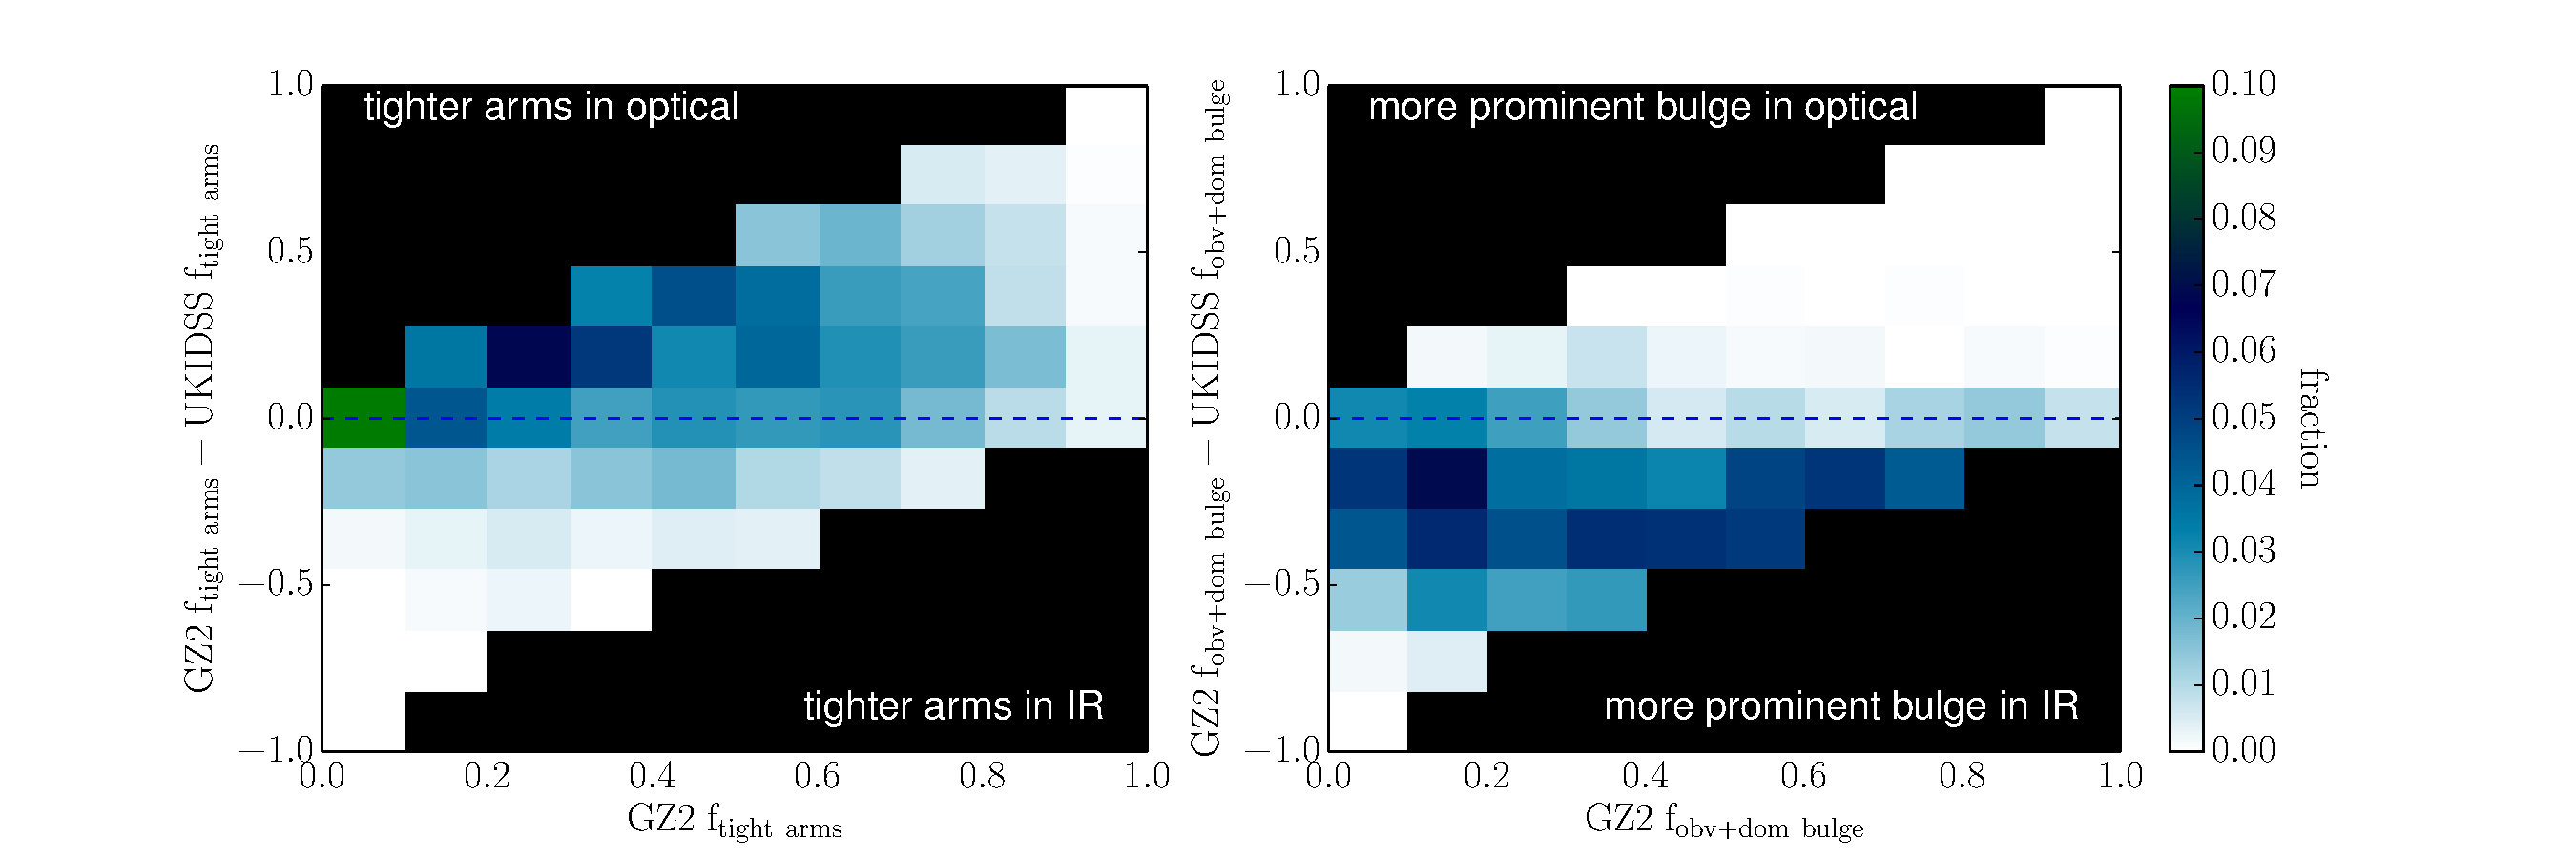
\includegraphics[width=1\textwidth,trim={4cm 0cm 4cm 0cm},clip]{figures/t_type.pdf}
\caption{IR images of galaxies tend to have a looser appearance of arms and more prominent bulges than in optical images. Shown is the difference between optical and IR $\rm f_{tight~arms}$ as a function of optical/GZ2 $\rm f_{tight~arms}$ (\textbf{left}), and difference between optical and IR $\rm f_{obv+dom}$ as a function of optical/GZ2 $\rm f_{obv+dom}$ (\textbf{right}) for 502 galaxies which were classified as spiral in both IR and optical images. The colors represent the fraction of galaxies that populate any given bin, and bins which could not represent a possible difference in vote fraction ($\Delta f > f$ or $\Delta f < f-1$) are colored black. The blue dotted line in both represents a difference in vote fraction of 0, such that galaxies above the line have larger IR vote fractions for the feature represented in each plot, respectively.}
\label{fig:ttype}
\end{figure}

So far the appearance of spiral arms visible in both the optical and infrared have been compared; on average, GZ infrared morphologies are slightly earlier than the optical, a result of a looser appearance of the arms and more prominant bulges. But what of the the optically spiral galaxies whose arms disappear in the IR? Of the 1,042 optical spirals in the volume and S/N limited sample, 540 (52\%) of these were not classified as spirals in the IR. These types will be hereafter referred to as SONIs (Spiral in Optical but Not Infrared) for convenience. The most common morphological classes of galaxies which do not exhibit spiral arms are ellipticals, S0s, and edge-on disks (which may or may not truly have spiral arms, but cannot be discerned due to orientation angle). This section will explore which of these classes SONIs tend to occupy in the IR. 

Figure~\ref{fig:sankey} shows the different pathways galaxies in the UKIDSS sample follow through the decision tree. The left flow diagram shows the breakdown of morphologies of all galaxies in the volume-limited sample, while the right diagram includes only the SONIs. Galaxies which follow the spiral pathway must first be classfied as featured (T00), then not edge-on (T01). At this point the not edge-on featured galaxies can follow the 'spiral' or 'not spiral' path (T03). Those marked as spirals are classified by how tight the arms appear (T09) and how many arms are present (T10). Last, both the spirals and not-spirals are classified by bulge prominence (T04). As a result of this type of decision tree, there are several pathways galaxies may take to ultimately obtain a ``not spiral'' classification. They may be classified from the beginning as not featured (as ellipticals or star/artifacts), or they may be featured but edge-on, or they may be featured and not edge-on, and still show no spiral arms.

The diagram on the right shows which of these paths SONIs tend to take, resulting in their ultimate classification of ``not spiral'' in the IR. 72\% of SONIs follow the elliptical path; that is, the optically-visible spiral arms must become so faint that all that can be seen is the central bulge, which by eye becomes discernable from a full spheroidal galaxy. 28\% are classified as both featured and not edge-on. One might hypothesize a majority of these exhibit stellar bars, which drives the ``featured'' classifications when there are no spiral arms to do so. However, there is no excess of strong bars detected; only 24\% of the not edge-on featured SONIs are strongly barred, which is actually lower than that of the full sample (33\%). Since the diagram flows are determined by a plurality of votes for each Task, however, the possibility of weak bars of driving the ``featured'' classification is not accounted for here. Therefore most of the galaxies on this path are likely either weakly barred, and/or retain evidence of both an underlying disk and a bulge, with enough contrast to keep them from being classified as purely elliptical. However it is clear that the bulge is very close to dominating the total light distribution in many of these galaxies; for SONIs, 90\% are classified as having an either obvious or dominant bulge, as compared to 83\% showing obvious or dominant bulges in the full sample. 



\begin{figure}
\centering
\includegraphics[width=1\textwidth]{figures/sankey.pdf}
\caption{Flow diagram showing the breakdown of morphologies in the UKIDSS sample. \textbf{Left}: 15,491 galaxies in the volume-limited sample. \textbf{Right}: 2,346 SONIs: galaxies which were classified as spiral in the optical GZ2 classifications but do not follow the spiral path in the UKIDSS classifications.}
\label{fig:sankey}
\end{figure}

\begin{figure}
\centering
\includegraphics[width=\textwidth,trim={5cm 1cm 5cm 1cm},clip]{figures/smooth_sonis.pdf}
\caption{Example images of galaxies which were classified as spiral in optical GZ2 classifications but followed the ``smooth'' path in the UKIDSS classifications.}
\label{fig:smooth}
\end{figure}

\begin{figure}
\centering
\includegraphics[width=\textwidth,trim={5cm 1cm 5cm 1cm},clip]{figures/notedgeon_sonis.pdf}
\caption{Example images of galaxies which were classified as spiral in optical GZ2 classifications but followed the ``featured, not edge-on, no spiral'' path in the UKIDSS classifications.}
\label{fig:notedgeon}
\end{figure}

 
\begin{figure}
\centering
\includegraphics[width=\textwidth,trim={5cm 1cm 5cm 1cm},clip]{figures/edgeon_sonis.pdf}
\caption{Example images of galaxies which were classified as spiral in optical GZ2 classifications but followed the ``featured, edge-on'' path in the UKIDSS classifications.}
\label{fig:edgeon}
\end{figure}

 
\begin{figure}
\centering
\includegraphics[width=\textwidth,trim={5cm 1cm 5cm 1cm},clip]{figures/artifact_sonis.pdf}
\caption{Example images of galaxies which were classified as spiral in optical GZ2 classifications but were classified as star/artifact in the UKIDSS classifications.}
\label{fig:artifact}
\end{figure}


\section{Bar Fraction}
This section will focus on the properties of bars observed in the two wavelengths: first by measuring the fraction of bars detected, and secondly the relative strengths. To avoid possible confusion in this portion of the text, two similar quanities are defined explicitely here: the \emph{bar fraction} is defined as the ratio of barred galaxies to total galaxies in a sample, and $\rm f_{bar}$ is the \emph{bar vote fraction}, which is the fraction of users who detected a bar in an image of an \emph{individual galaxy}.

To measure the fraction of barred galaxies, the sample is first limited to galaxies for which there were at least 20 answers to the question in the decision tree that asks, ``Is there a sign of a bar feature through the center of the galaxy?'' This cut serves two purposes: first, it provites good statistics in computing $\rm f_{bar}$ for each galaxy (see Figure stats). Second, for the UKIDSS sample which has at maximum 40 total classifications per galaxy, this places an indirect cut on the preceding vote fractions $\rm f_{features} \ge 0.5$ and $\rm f_{not~edge~on} \ge 0.5$. This intrinsically limits the sample to featured, not edge-on galaxies, which is precisely the sample desired for computing the bar fraction, as bars are nonexistant in elliptical galaxies, or indetectable in highly-inclined edge-on galaxies. For the GZ2 sample, however, a significant portion of the galaxies have between 40-60 total classifications; so, a cut of $\rm N_{bar} \ge 20$ would not guarantee the same minima for the preceding vote fractions. Therefore direct cuts of $\rm f_{features} \ge 0.5$ and $\rm f_{not~edge~on}$ are additionally placed on the GZ2 classifications to ensure the same sample selection for both wavelengths.  

\begin{figure}
\centering
\includegraphics[width=\textwidth]{figures/ubar_vs_gbar.pdf}
\caption{Dotted lines indicate the threshold for bar classification; $f_{bar}>0.3$. Galaxies shown had at least 20 people answering the bar question. }
\label{fig:ubarvgbar}
\end{figure}

Figure~\ref{fig:ubarvgbar} compares $\rm f_{bar}$ measured in the UKIDSS and GZ2 images for galaxies which were classified as featured and not edge-on in both samples. In this study, any galaxy for which $\rm f_{bar} \ge 0.3$ is classified as barred. The dashed lines in the figure mark this threshold, such that galaxies to the right of the vertical dashed line were classified as barred in the optical images, and those above the horizontal dashed line were classified as barred in the IR images. Four regions can be defined in this way: The top right region of the plot represents galaxies classified as barred in both wavelenths, the bottom right shows those which are unbarred in both, the top left shows those which are barred in the IR but not the optical, and the bottom right shows those which are barred in the optical but not IR.  


\begin{figure}
\centering
\includegraphics[width=\textwidth,trim={5cm 1cm 5cm 1cm},clip]{figures/ubar_no_gzbar.pdf}
\caption{Galaxies classified as barred in optical GZ2 and unbarred in infrared UKIDSS.}
\label{fig:ubarnogbar}
\end{figure}

\begin{figure}
\centering
\includegraphics[width=\textwidth,trim={5cm 1cm 5cm 1cm},clip]{figures/gzbar_no_ubar.pdf}
\caption{Galaxies classified as barred in infrared UKIDSS and unbarred in optical GZ2.}
\label{fig:gbarnoubar}
\end{figure}


